%-------------------------------------------------------------------------------
%                            BAB II
%               TINJAUAN PUSTAKA DAN DASAR TEORI
%-------------------------------------------------------------------------------

\chapter{TINJAUAN PUSTAKA DAN DASAR TEORI}                

\section{Tinjauan Pustaka}
  Secara umum, cara untuk menghubungkan WSN dengan jaringan internet dapat dikelompokkan menjadi dua. Cara pertama adalah menggunakan gateway dan cara yang kedua adalah dengan menggunakan simpul sensor yang sudah dilengkapi dengan protokol internet. Cara yang lebih mudah ditempuh adalah dengan cara yang pertama karena pengubahan yang dilakukan relatif tidak terlalu besar. Sedangkan cara yang kedua akan menemui banyak kendala terutama pada WSN yang sudah terpasang karena harus dilakukan penggantian tiap simpul sensor.

  Salah satu usaha untuk mengintegrasikan jaringan WSN dengan jaringan WiFi menggunakan gateway misalnya dilakukan pada penelitian. Pada riset tersebut pengintegrasian dilakukan dengan sebuah komputer yang didedikasikan untuk keperluan tertentu. Penggunaan komputer khusus ini adalah hardware-solution yang membutuhkan biaya dan kerumitan sistem.

  Riset pada juga menawarkan pengintegrasian dengan jaringan IP. Namun demikian di dalam riset ini diperlukan perubahan yang signifikan jika konfigurasi jaringan sensor nirkabel sudah terpasang. Simpul sensor yang digunakan harus diganti dengan simpul sensor yang mendukung IP. Hal ini jelas akan memakan biaya yang cukup besar dan tidak praktis untuk dilakukan. Terlebih lagi jika jumlah sensor yang terpasang jumlahnya cukup banyak.

  Riset pada sudah berhasil mengembangkan sebuah AP menjadi gateway yang dapat digunakan untuk menghubungkan sebuah protokol WSN dengan jaringan IP. Protokol WSN yang digunakan adalah protokol dari IQRF. Penelitian tersebut kemudian dilanjutkan dengan penelitian yang sudah diterapkan dalam sistem domotic.

\section{Landasan Teori}
  \subsection{\emph{Wireless Sensor Network}}
    Jaringan sensor nirkabel (Wireless Sensor Network, WSN) adalah jaringan simpul sensor otonom yang terdistribusi digunakan untuk memonitor kondisi fisik atau lingkungan misalnya suhu, suara, getaran, kelembaban, dan lain-lain. Selain itu, tidak menutup kemungkinan untuk menambahkan fungsi tambahan pada setiap simpul misalnya port masukan/keluaran (I/O port) yang terdapat dalam setiap simpul dihubungkan dengan aktuator sehingga dapat digunakan untuk mengendalikan piranti elektrik atau elektronis.

    Secara umum, WSN dapat diilustrasikan seperti Gambar \ref{wsn}. Pada gambar tersebut terlihat adanya beberapa simpul yang diwakili dengan titik berukuran kecil dan satu buah simpul yang diwakili dengan titik berukuran lebih besar. Titik yang berukuran kecil mewakili simpul sensor sedangkan titik yang berukuran besar mewakili gateway yang berfungsi menghubungkan jaringan sensor nirkabel dengan pengendali utama yang dalam gambar tersebut diwakili oleh sebuah komputer. Contoh sebuah simpul dari IQRF ditunjukkan pada Gambar \ref{iqrf}.

      \begin{figure}[ht!]
        \centering
          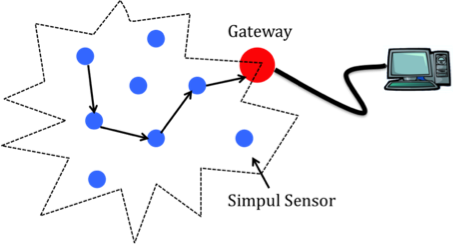
\includegraphics{gambar/wsn}
          \caption{Jaringan sensor nirkabel.}
          \label{wsn}
      \end{figure}

    Pada umumnya, WSN adalah jaringan yang berdiri sendiri. Untuk menghubungkan WSN dengan jaringan yang lain misalnya jaringan internet, maka salah satu cara adalah dengan membangun gateway WSN yang mampu menjembatani perbedaan protokol yang ada pada WSN dan jaringan internet. Cara tersebut adalah cara yang ditempuh dalam penelitian ini karena lebih mudah dilakukan dibandingkan dengan cara yang lain seperti sudah dijelaskan pada Bab Tinjauan Pustaka.

      \begin{figure}[ht!]
        \centering
          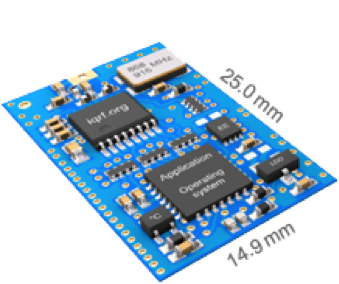
\includegraphics{gambar/iqrf}
          \caption{Contoh sebuah simpul sensor IQRF.}
          \label{iqrf}
      \end{figure}

    Sementara itu, jaringan WiFi sebagai jaringan lokal nirkabel yang digunakan untuk komunikasi data dalam suatu area lokal dan sudah tersebar di berbagai tempat. Lokal yang dimaksud disini adalah area yang tidak terlalu luas yaitu dengan radius sekitar 20m atau dalam sebuah gedung. Untuk membangun jaringan lokal menggunakan WiFi, perangkat utama yang digunakan adalah Access Point (AP). AP adalah piranti yang akan menjadi koordinator dalam jaringan lokal jika diinginkan topologi bintang (star) seperti diilustrasikan pada Gambar \ref{star}.

      \begin{figure}[ht!]
        \centering
          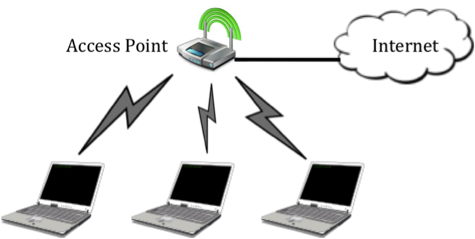
\includegraphics{gambar/star}
          \caption{Jaringan bintang menggunakan WiFi.}
          \label{star}
      \end{figure}

    Gambar \ref{star} memberi ilustrasi sebuah jaringan WiFi yang terdiri dari tiga buah komputer dan satu buah AP yang terhubung ke jaringan internet. Dengan konfigurasi tersebut, semua komputer yang ada di dalam jaringan WiFi dapat berkomunikasi dengan internet dengan aturan yang ditentukan oleh AP.

    Jika dilihat lebih dalam lagi, AP ini sebenarnya adalah piranti tertanam (embedded device) yang didalamnya sudah terdapat pusat pengolahan utama, memory, dan penyimpanan (storage). Dengan kenyataan inilah maka AP mempunyai potensi untuk menjagi gateway bagi jaringan WiFi dan WSN ke jaringan internet. Untuk mengembangkan aplikasi yang akan ditanamkan ke dalam AP, maka diperlukan sistem operasi yang sesuai untuk AP.

  \subsection{IQRF}
    IQRF adalah teknologi komunikasi nirkabel berbasis paket melalui frekuensi radio dalam pita frekuensi sub-GHz. Teknologi ini dimaksudkan untuk penggunaan umum saat konektivitas nirkabel dibutuhkan, entah \emph{point to point} atau jaringan yang kompleks. fungsionalitas lengkapnya bergantung semata-mata pada aplikasi berbahasa C yang ditulis oleh pengguna.

    Peranti kominikasi dasar dari IQRF adalah sebuah modul pancar-rima termasuk unit mikrokontroler dengan sistem operasi tertanam yang mengimplementasikan lapisan \emph{link} dan lapisan jaringan yang mendukung jaringan jala (\emph{mesh}) dengan protokol IQMESH. Tidak ada tingkat komunikasi yang lebih tinggi seperti lapisan \emph{transport} yang termasuk kedalam teknologi ini.

    Fitur-fitur yang dimiliki antara lain:
      \begin{itemize}
        \item Kecepatan, daya, dan ukuran data yang rendah,
        \item RF yang berbasis paket data, maksimal 128 Byte per paket,
        \item pita frekuensi sub-GHz (868 MHz, 916 MHz, dst.), \emph{multichannel}, dan modulasi FSK,
        \item \emph{bit rate} 1.2 kb/s – 86.2 kb/s,
        \item daya keluaran maksimal 20 mW,
        \item maksimal 65.000 peranti dalam satu jaringan,
        \item konsumsi daya yang rendah: 380 nA saat \emph{standby}, 25 µA saat menerima.
      \end{itemize}


  \subsection{XBee}
    XBee adalah sebuah merk dari Digi International untuk keluarga modul radio. XBee pertama diperkenalkan dalam merk MaxStream pada tahun 2005 yang berdasarkan pada standar IEEE 802.15.4-2003 untuk \emph{point to point} dan komunikasi bintang dalam \emph{baud rate} 250 kbit/s.

      \begin{figure}[ht!]
        \centering
          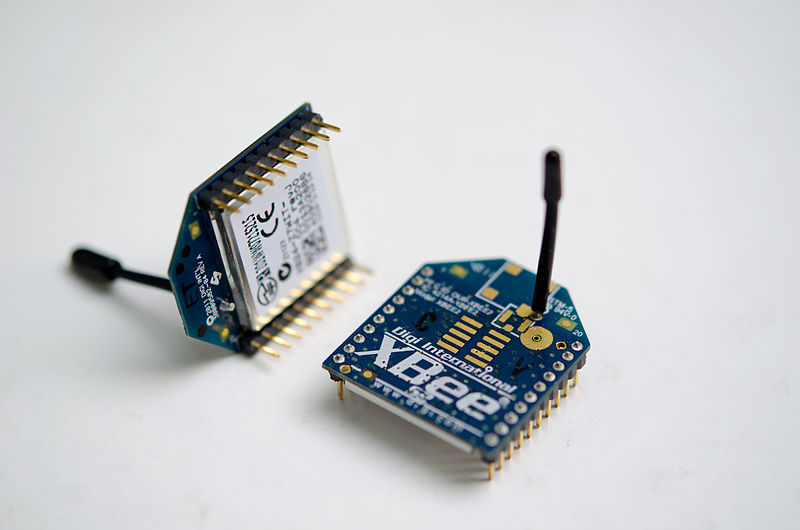
\includegraphics{gambar/xbee}
          \caption{Sepasang peranti XBee.}
          \label{xbee}
      \end{figure}

    Pada awalnya diperkenalkan dua model, yaitu 1mW XBee dan 100mW XBee-PRO. Sejak pertama kali diperkenalkan, beberapa buah XBee baru juga diperkenalkan dan semua XBee sekarang dipasarkan dengan merk Digi. Contoh peranti XBee dapat dilihat pada Gambar \ref{xbee}.

  \subsection{TCP/IP}
    Protokol internet adalah kumpulan protokol-protokol komunikasi yang digunakan dalam internet dan jaringan komputer sejenis, dan umumnya merupakan protokol yang paling populer untuk WAN. Pada umumnya hal ini dikenal dengan TCP/IP, karena protokol utamanya merupakan protokol jaringan pertama yang terstandarisasi. Terkadang hal ini dikenal dengan model DoD karena pengaruh ARPANET pada dekade 1970an.

    TCP/IP menyediakan konektivitas antar ujung yang menspesifikasikan bagaimana data harus diformat, dialamatkan, ditransmisikan, dirutekan, dan diterima di tujuan. TCP/IP memiliki empat layer abstraksi yang digunakan untuk mengurutkan semua protokol internet menurut jangkauan jaringan yang terlibat. Dari terendah sampai tertinggi, lapisan-lapisan tersebut adalah layer link, layer internet, layer transport, dan layer aplikasi.

  \subsection{\emph{Access Point}}
    \emph{Access Point}, disingkat AP, atau juga dikenal dengan istilah \emph{Wireless Access Point} adalah sebuah peranti yang memungkinkan peranti-peranti nirkabel untuk terkoneksi dengan jaringan kabel menggunakan Wi-Fi atau standar lain. AP biasanya terkoneksi dengan sebuah \emph{router} (melalui jaringan kabel) sebagai peranti yang berdiri sendiri, namun juga dapat menjadi bagian dalam komponen \emph{router} tersebut.

    Penggunaan secara korporat melibatkan beberapa AP ke dalam jaringan kabel dan menyediakan akses nirkabel ke LAN kantor. AP diatur dengan WLAN \emph{Controller} yang menangani pengaturan daya RF, kanal-kanal, autentikasi, dan keamanan.
    
    Sebuah \emph{hotspot} adalah aplikasi dari satu atau beberapa AP, di mana peranti dapat terhubung ke Internet dengan mudah. Konsep ini sudah menjadi hal yang umum di beberapa kota besar, di mana kombinasi dari warung kopi, perpustakaan, dan AP milik pribadi memungkinkan klien untuk terkoneksi dengan Internet. Koleksi dari \emph{hotspot} yang terkoneksi dapat disebut sebagai sebuah jaringan \emph{lili pad}.

  \subsection{Web Server}
    Web server dapat mengacu pada perangkat keras atau perangkat lunak yang membantu dalam penyampaian konten web yang dapat diakses melalui internet.

    Penggunaan web server yang paling umum adalah sebagai host untuk halaman web, walaupun ada beberapa penggunaan lain seperti game, media penyimpan data, atau penjalanan aplikasi perusahaan.


  \subsection{AJAX}
    AJAX adalah kelompok dari teknik-teknik pengembangan web yang digunakan pada klien untuk membuat aplikasi asinkron. Dengan AJAX, aplikasi web dapat mengirim dan menerima data dari sebuah server secara asinkron tanpa mengganggu tampilan dari halaman yang ada. Data dapat diambil menggunakan obyek XMLHttpRequest. Penggunaan XML tidak diperlukan, malahan JSON lebih sering digunakan, dan rekues tidak harus asinkron.

    AJAX bukanlah sebuah teknologi, tapi kelompok dari teknologi-teknologi. HTML dan CSS dapat digunakan dalam kombinasi untuk mark up dan informasi tampilan. DOM diakses oleh JavaScript untuk menampilkan dan mengijinkan pengguna untuk berinteraksi dengan informasi tertampil. JavaScript dan obyek XMLHttpRequest menyediakan sebuah metode untuk pertukaran data secara asinkron antara browser dan server untuk menghindari muat ulang halaman secara keseluruhan.


  \subsection{OpenWRT}
    OpenWRT adalah sebuah sistem operasi untuk \emph{embedded device} yang berbasis pada Linux kernel. OpenWRT pada umumnya digunakan dalam routing \emph{network traffic}. Komponen-komponen utamanya adalah Linux kernel, util-linux, uClibc dan BusyBox. Semua komponen sudah dioptimalkan dan dimampatkan untuk bisa muat dalam \emph{router} rumahan yang memiliki keterbatasan media penyimpan dan memori. OpenWRT dapat dikonfigurasikan melalui antarmuka \emph{command-line} (\emph{ash shell}), seperti dapat dilihat pada Gambar \ref{openwrt}, atau dengan antarmuka Web (LuCI). Terdapat kurang lebih 3.500 paket-paket perangkat lunak tambahan yang tersedia untuk diinstal melalui sistem manajemen paket \emph{opkg}.

      \begin{figure}[ht!]
        \centering
          
\includegraphics[width=10cm]{gambar/openwrt}
          \caption{Tampilan antarmuka \emph{command-line} OpenWRT versi \emph{BackFire}.}
          \label{openwrt}
      \end{figure}

    OpenWRT dapat berjalan pada router CPE (\emph{Customer Premised Equipment}), \emph{gateway} residensial, komputer saku (seperti Ben NanoNote), dan komputer jinjing. OpenWRT juga dapat berjalan pada komputer konvensional atau komputer dengan arsitektur x86. Banyak \emph{patch} dari kode sesumber berbasis OpenWRT yang diubah kedalam Linux kernel utama.

  \subsection{SSHFS}
    SSHFS (SSH Filesystem) adalah sebuah klien \emph{filesystem} untuk \emph{mount} dan berinteraksi dengan direktori dan arsip yang berlokasi pada server atau \emph{workstation}. Klien berinteraksi dengan server dengan SSH \emph{File Transfer Protocol} (SFTP), sebuah protokol jaringan yang menyediakan akses ke arsip, transfer arsip, dan fungsionalitas manajemen arsip melalui aliran data yang didesain sebagai ekstensi dari protokol SSH versi 2.0.

  \subsection{Bootstrap}
    Bootstrap adalah koleksi gratis dari alat-alat untuk membuat situs web dan aplikasi berbasis web. Bootstrap terdiri dari HTML dan contoh desain berbasis CSS untuk tipografi, borang, tombol, navigasi, komponen antarmuka lain, dan juga ekstensi JavaScript yang bersifat opsional.

    Bootstrap merupakan proyek paling populer pada GitHub, dan sudah digunakan oleh, diantaranya, NASA dan MSNBC.
